% Compatibility shims for the local hyperref/LaTeX combination.
\providecommand\IfDocumentMetadataT[1]{}
\providecommand\IfDocumentMetadataTF[2]{#2}
\documentclass[aspectratio=169,9pt]{beamer}
\newcommand{\qxdecklabel}{Quispe \& Xu (2026) · Lean formalization companion}
\NeedsTeXFormat{LaTeX2e}
\RequirePackage{fontspec}
\RequirePackage{amsmath,amssymb,mathtools}
\RequirePackage{booktabs}
\RequirePackage{graphicx}
\RequirePackage{microtype}
\RequirePackage{ragged2e}
\RequirePackage{hyperref}
\RequirePackage{tikz}
\usetikzlibrary{arrows.meta,positioning,calc}

\IfFontExistsTF{Avenir Next}{\setsansfont{Avenir Next}}{\setsansfont{TeX Gyre Heros}}

\definecolor{QXNavy}{HTML}{0C2852}
\definecolor{QXRed}{HTML}{982A34}
\definecolor{QXGraphite}{HTML}{20242A}
\definecolor{QXMuted}{HTML}{5B6470}
\definecolor{QXRedTitle}{HTML}{F4E8EA}
\definecolor{QXRedBody}{HTML}{F9F5F5}
\definecolor{QXBlueTitle}{HTML}{EBEEF1}
\definecolor{QXBlueBody}{HTML}{F5F6F8}
\definecolor{QXGreen}{HTML}{3B5526}
\definecolor{QXDivider}{HTML}{D9DEE4}

\usetheme{default}
\usefonttheme{professionalfonts}
\setbeamertemplate{navigation symbols}{}
\setbeamersize{text margin left=0.54cm,text margin right=0.54cm}
\setbeamercolor{background canvas}{bg=white}
\setbeamercolor{normal text}{fg=QXGraphite,bg=white}
\setbeamercolor{frametitle}{fg=white,bg=QXNavy}
\setbeamercolor{structure}{fg=QXNavy}
\setbeamercolor{alerted text}{fg=QXRed}
\setbeamercolor{qx red title}{fg=QXRed,bg=QXRedTitle}
\setbeamercolor{qx red body}{fg=QXGraphite,bg=QXRedBody}
\setbeamercolor{qx blue title}{fg=QXNavy,bg=QXBlueTitle}
\setbeamercolor{qx blue body}{fg=QXGraphite,bg=QXBlueBody}
\setbeamercolor{qx accent line}{bg=QXRed}
\setbeamercolor{qx divider line}{bg=QXDivider}
\setbeamercolor{qx foot}{fg=QXMuted,bg=white}
\setbeamercolor{qx takeaway}{fg=white,bg=QXNavy}
\setbeamercolor{qx placeholder}{fg=QXMuted,bg=QXBlueBody}
\setbeamerfont{frametitle}{size=\large,series=\bfseries}
\setbeamerfont{block title}{size=\normalsize,series=\bfseries}
\setbeamerfont{footline}{size=\scriptsize}
\providecommand{\qxdecklabel}{Quispe \& Xu (2026) · language-frontier audit}

\setbeamertemplate{frametitle}{%
  \nointerlineskip
  \begin{beamercolorbox}[wd=\paperwidth,ht=0.62cm,dp=0.23cm,leftskip=0.48cm]{frametitle}%
    \usebeamerfont{frametitle}\insertframetitle
  \end{beamercolorbox}%
  \nointerlineskip
  \hbox{%
    \begin{beamercolorbox}[wd=1.05cm,ht=0.018cm,dp=0cm]{qx accent line}\end{beamercolorbox}%
    \begin{beamercolorbox}[wd=\dimexpr\paperwidth-1.05cm\relax,ht=0.018cm,dp=0cm]{qx divider line}\end{beamercolorbox}%
  }%
}

\setbeamertemplate{footline}{%
  \leavevmode\hbox{%
    \begin{beamercolorbox}[wd=.83\paperwidth,ht=0.26cm,dp=0.10cm,leftskip=.52cm]{qx foot}%
      \qxdecklabel
    \end{beamercolorbox}%
    \begin{beamercolorbox}[wd=.17\paperwidth,ht=0.26cm,dp=0.10cm,rightskip=.52cm plus1fil]{qx foot}%
      \insertframenumber/\inserttotalframenumber
    \end{beamercolorbox}%
  }%
}

\newcommand{\E}{\mathbb{E}}
\newcommand{\ATT}{\operatorname{ATT}}
\newcommand{\qxredblock}[2]{%
  \begin{beamercolorbox}[wd=\linewidth,sep=0.10cm,leftskip=0.07cm,rightskip=0.07cm]{qx red title}\usebeamerfont{block title}#1\end{beamercolorbox}%
  \nointerlineskip
  \begin{beamercolorbox}[wd=\linewidth,sep=0.13cm,leftskip=0.10cm,rightskip=0.10cm]{qx red body}#2\end{beamercolorbox}%
}
\newcommand{\qxblueblock}[2]{%
  \begin{beamercolorbox}[wd=\linewidth,sep=0.10cm,leftskip=0.07cm,rightskip=0.07cm]{qx blue title}\usebeamerfont{block title}#1\end{beamercolorbox}%
  \nointerlineskip
  \begin{beamercolorbox}[wd=\linewidth,sep=0.13cm,leftskip=0.10cm,rightskip=0.10cm]{qx blue body}#2\end{beamercolorbox}%
}
\newcommand{\qxtwocol}[4]{%
  \noindent\hspace*{0.12cm}%
  \begin{minipage}[t]{#1\linewidth}\vspace{0pt}#2\end{minipage}%
  \hfill
  \begin{minipage}[t]{#3\linewidth}\vspace{0pt}#4\end{minipage}%
  \hspace*{0.12cm}\par
}
\newcommand{\qxtakeaway}[1]{%
  \begin{beamercolorbox}[wd=\linewidth,sep=0.12cm,leftskip=0.10cm,rightskip=0.10cm]{qx takeaway}
    \small\bfseries #1
  \end{beamercolorbox}%
}

\title{How I Used Lean for Agentic Delegation and the Language Frontier of Software Developers: A Model and Evidence from Claude Code on GitHub}
\author{Gabriel Saco}
\hypersetup{
  pdftitle={How I Used Lean for Agentic Delegation and the Language Frontier of Software Developers: A Model and Evidence from Claude Code on GitHub},
  pdfauthor={Gabriel Saco}
}

\begin{document}

% 1
\begin{frame}[plain]
  \setbeamertemplate{footline}{}
  \vspace*{0.66cm}
  {\fontsize{14.7}{17.2}\selectfont\bfseries
    How I Used Lean for\par
    Agentic Delegation and the Language Frontier\par
    of Software Developers: A Model and Evidence\par
    from Claude Code on GitHub\par}
  \vspace{0.18cm}
  {\fontsize{10.8}{13.0}\selectfont
    Source translation, machine-checked proofs, a boundary counterexample,
    and an honest partial-formalization verdict\par}
  \vspace{0.28cm}
  {\color{QXRed}\rule{\linewidth}{0.55pt}}
  \vspace{0.38cm}
  {\normalsize\bfseries Gabriel Saco\par}
  \vspace{0.05cm}
  {\normalsize September 2, 2026\par}
  \vspace{0.16cm}
  {\small Universidad del Pac\'ifico\par}
  \vspace{0.18cm}
  {\small\color{QXMuted}
    Formalization of Quispe \& Xu (2026), arXiv:2605.25438v2\par}
  \vspace{0.08cm}
  {\small\href{https://github.com/gsaco/ai-03-quispe/tree/branch1}{\color{QXNavy}\ttfamily
    github.com/gsaco/ai-03-quispe/tree/branch1}\par}
  \vfill
  {\scriptsize\color{QXMuted}AI Economic Modeling\hfill Lean-focused companion\par}
\end{frame}

% 2
\begin{frame}[t]{What I asked Lean to do}
  \vspace{0.30cm}
  \begin{columns}[T,onlytextwidth]
    \begin{column}{0.48\textwidth}
      \qxblueblock{Mathematical question}{%
        \small Do the five named propositions follow from their stated
        threshold, ordering, finiteness, and monotonicity conditions?
      }
      \vspace{0.22cm}
      \qxredblock{Translation question}{%
        \small Does the Lean statement preserve the paper's domain,
        quantifiers, endpoints, inequalities, and conclusion?
      }
    \end{column}
    \begin{column}{0.48\textwidth}
      \qxredblock{Stress test}{%
        \small Are any strict claims false at an admissible boundary, or true
        only after adding a premise that the source does not state?
      }
      \vspace{0.22cm}
      \qxblueblock{Not the question}{%
        \small Lean cannot establish that Claude adoption is exogenous, that
        GitHub measurement is correct, or that an event-study coefficient is
        causal merely by proving the model's algebra.
      }
    \end{column}
  \end{columns}
  \vspace{0.28cm}
  \qxtakeaway{The target is a faithful implication: source assumptions in, source conclusion out.}
\end{frame}

% 3
\begin{frame}[t]{Source pinning and formal scope}
  \vspace{0.24cm}
  \begin{columns}[T,onlytextwidth]
    \begin{column}{0.54\textwidth}
      \qxblueblock{Pinned source}{%
        \small
        \textbf{Paper:} \emph{Agentic Delegation and the Language Frontier of
        Software Developers: A Model and Evidence from Claude Code on GitHub}

        \vspace{0.08cm}
        \textbf{Version:} arXiv v2, July 7, 2026

        \vspace{0.08cm}
        \textbf{SHA-256:}\par
        {\fontsize{6.4}{7.3}\selectfont\ttfamily
        cddc048711c43022d5fd01b995bfb111\par
        4c728c8c879b809b5fdc354a391d3c35\par}
      }
    \end{column}
    \begin{column}{0.42\textwidth}
      \qxredblock{Inventory before proving}{%
        \small
        \begin{itemize}\itemsep0.09cm
          \item three numbered assumptions;
          \item five numbered propositions;
          \item exact PDF locations;
          \item one source-facing \texttt{Spec} per proposition.
        \end{itemize}
      }
      \vspace{0.20cm}
      \qxblueblock{Deliberately out of scope}{%
        \footnotesize Empirical tables and figures, the event-study estimator,
        Bayesian learning, treatment detection, and causal identification.
      }
    \end{column}
  \end{columns}
  \vspace{0.24cm}
  \qxtakeaway{I formalized the pinned source directly; the worked example was a workflow guide, not a code source.}
\end{frame}

% 4
\begin{frame}[t]{The EconCSLib workflow I followed}
  \vspace{0.34cm}
  \begin{center}
    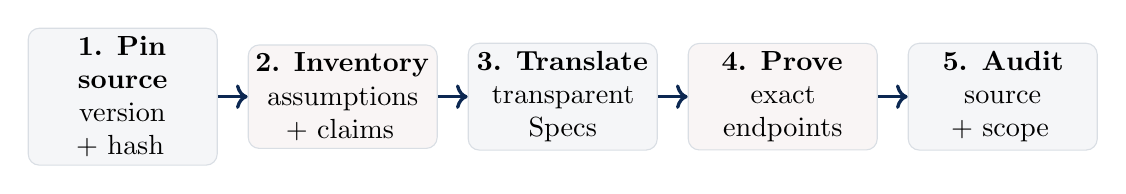
\begin{tikzpicture}[
      node distance=.38cm,
      box/.style={draw=QXDivider,rounded corners,minimum height=1.08cm,
        text width=2.20cm,align=center,inner sep=.10cm},
      arrow/.style={->,very thick,QXNavy}
    ]
      \node[box,fill=QXBlueBody] (pin) {\textbf{1. Pin source}\\version + hash};
      \node[box,fill=QXRedBody,right=of pin] (inventory) {\textbf{2. Inventory}\\assumptions + claims};
      \node[box,fill=QXBlueBody,right=of inventory] (spec) {\textbf{3. Translate}\\transparent Specs};
      \node[box,fill=QXRedBody,right=of spec] (prove) {\textbf{4. Prove}\\exact endpoints};
      \node[box,fill=QXBlueBody,right=of prove] (audit) {\textbf{5. Audit}\\source + scope};
      \draw[arrow] (pin)--(inventory);
      \draw[arrow] (inventory)--(spec);
      \draw[arrow] (spec)--(prove);
      \draw[arrow] (prove)--(audit);
    \end{tikzpicture}
  \end{center}
  \vspace{0.40cm}
  \begin{columns}[T,onlytextwidth]
    \begin{column}{0.47\textwidth}
      \qxredblock{Why statement first?}{%
        \small A proof of the wrong theorem is still a formalization failure.
        The paper-facing proposition is frozen before proof implementation.
      }
    \end{column}
    \begin{column}{0.47\textwidth}
      \qxblueblock{Why audit after proof?}{%
        \small Compilation checks logic. The audit checks whether stronger
        assumptions, weaker conclusions, or changed domains entered silently.
      }
    \end{column}
  \end{columns}
\end{frame}

% 5
\begin{frame}[t]{Four layers keep meaning separate from proof engineering}
  \vspace{0.22cm}
  \begin{columns}[T,onlytextwidth]
    \begin{column}{0.56\textwidth}
      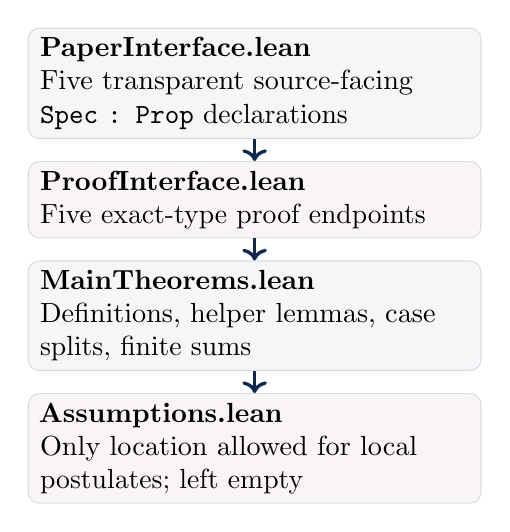
\begin{tikzpicture}[
        node distance=.28cm,
        box/.style={draw=QXDivider,rounded corners,minimum height=.76cm,
          text width=5.45cm,align=left,inner xsep=.15cm},
        arrow/.style={->,very thick,QXNavy}
      ]
        \node[box,fill=QXBlueBody] (spec) {\textbf{PaperInterface.lean}\\Five transparent source-facing \texttt{Spec : Prop} declarations};
        \node[box,fill=QXRedBody,below=of spec] (endpoint) {\textbf{ProofInterface.lean}\\Five exact-type proof endpoints};
        \node[box,fill=QXBlueBody,below=of endpoint] (impl) {\textbf{MainTheorems.lean}\\Definitions, helper lemmas, case splits, finite sums};
        \node[box,fill=QXRedBody,below=of impl] (assume) {\textbf{Assumptions.lean}\\Only location allowed for local postulates; left empty};
        \draw[arrow] (spec)--(endpoint);
        \draw[arrow] (endpoint)--(impl);
        \draw[arrow] (impl)--(assume);
      \end{tikzpicture}
    \end{column}
    \begin{column}{0.40\textwidth}
      \qxblueblock{Human review surface}{%
        \small Read \texttt{PaperInterface.lean} first. It exposes the formal
        claim without proof tactics obscuring its meaning.
      }
      \vspace{0.16cm}
      \qxredblock{Audit surface}{%
        \small The JSON ledgers map source locations to Specs, classify scope
        gaps, and quarantine the Proposition 3 defect.
      }
      \vspace{0.16cm}
      \qxblueblock{Visual dependency map}{%
        \small \texttt{docs/DependencyDAG.pdf} links the three assumptions to
        the propositions they support.
      }
    \end{column}
  \end{columns}
\end{frame}

% 6
\begin{frame}[t]{Formal theorem inventory}
  \vspace{0.18cm}
  {\small
  \begin{tabular}{@{}p{.15\linewidth}p{.36\linewidth}p{.39\linewidth}@{}}
    \toprule
    \textbf{Source} & \textbf{Lean endpoint} & \textbf{Status and scope} \\
    \midrule
    Prop. 1 & \texttt{frontierExpansion} &
      Proved: static menu and finite language count. \\
    Prop. 2 & \begin{tabular}[t]{@{}l@{}}\texttt{activationBandFor}\\[-0.03cm]
      \texttt{UnfamiliarLanguages}\end{tabular} &
      Proved with an order-theoretic CDF abstraction. \\
    Prop. 3 & \begin{tabular}[t]{@{}l@{}}\texttt{dynamicCumulative}\\[-0.03cm]
      \texttt{LanguageEffectCorrected}\end{tabular} &
      Corrected theorem proved; printed endpoint refuted. \\
    Prop. 4 & \texttt{specialistAndAbilityHeterogeneity} &
      Proved under explicit nonnegativity and monotonicity premises. \\
    Prop. 5 & \texttt{repositoryExpansion} &
      Proved pointwise for a finite repository type. \\
    \bottomrule
  \end{tabular}}\par
  \vspace{0.34cm}
  \qxblueblock{Logical result}{%
    \small All five exact-type endpoints compile without proof holes. Every
    economic restriction appears in the theorem signature or in a transparent
    source-facing specification.
  }
  \vspace{0.22cm}
  \qxredblock{Semantic result}{%
    \small Four targets preserve the finite core of the source claim. The fifth,
    Proposition 3, requires an explicit domain correction and therefore prevents
    a fully formalized label.
  }
\end{frame}

% 7
\begin{frame}[t]{Proposition 1: adding a mode cannot shrink the frontier}
  \setlength{\abovedisplayskip}{0.20em}
  \setlength{\belowdisplayskip}{0.20em}
  \vspace{0.12cm}
  \qxblueblock{1 · Paper mathematics}{%
    \small
    \[
      \max\{V^S,V^C,V^D\}\ge\max\{V^S,V^C\}
      \quad\Longrightarrow\quad
      Z^2_{ikt}\ge Z^1_{ikt},\qquad N^2_{it}\ge N^1_{it}.
    \]
  }
  \vspace{0.12cm}
  \begin{columns}[T,onlytextwidth]
    \begin{column}{0.55\textwidth}
      \qxredblock{2 · Lean proof core}{%
        {\fontsize{6.5}{7.5}\selectfont\ttfamily
        theorem frontierExpansionProof\par
        \ \ \{Language : Type\} [Fintype Language]\par
        \ \ (oldSurplus delegationSurplus : Language -> Real) :\par
        \ \ (forall k, oldActive k <= newActive k) /\textbackslash\par
        \ \ \ \ sum oldActive <= sum newActive := by\par
        \quad have hpoint : forall k, oldActive k <= newActive k := by\par
        \qquad intro k\par
        \qquad by\_cases hold : 0 <= oldSurplus k\par
        \qquad . exact hold.trans (le\_max\_left \_ \_)\par
        \quad exact <hpoint, Finset.sum\_le\_sum ...>\par}
      }
    \end{column}
    \begin{column}{0.43\textwidth}
      \qxblueblock{3 · Interpretation}{%
        \footnotesize Languages form an arbitrary finite type. Lean first proves
        the indicator inequality for each language, then lifts it to the total
        count with \texttt{Finset.sum\_le\_sum}.
      }
      \vspace{0.10cm}
      \qxredblock{Exactness}{%
        \footnotesize This verifies the pathwise static menu result. It does not
        prove that delegation is adopted, strictly preferred, or empirically
        responsible for observed expansion.
      }
    \end{column}
  \end{columns}
\end{frame}

% 8
\begin{frame}[t]{Proposition 2: translating the activation band}
  \setlength{\abovedisplayskip}{0.18em}
  \setlength{\belowdisplayskip}{0.18em}
  \vspace{0.08cm}
  \qxblueblock{1 · Paper equation}{%
    \small Under the no-foothold condition and $T^D<T^S$,
    \[
      Z^2-Z^1=\mathbb I\{T^D\le\omega<T^S\},
      \qquad
      \Pr(Z^2-Z^1=1)=F(T^S)-F(T^D).
    \]
  }
  \vspace{0.10cm}
  \begin{columns}[T,onlytextwidth]
    \begin{column}{0.55\textwidth}
      \qxredblock{2 · Lean statement}{%
        {\fontsize{6.4}{7.35}\selectfont\ttfamily
        theorem activationBandIndicator\par
        \ \ (TD TS opportunity : Real)\par
        \ \ (hthreshold : TD < TS) :\par
        \ \ (if TD <= opportunity then 1 else 0) -\par
        \ \ \ \ (if TS <= opportunity then 1 else 0) =\par
        \ \ if TD <= opportunity /\textbackslash\ opportunity < TS\par
        \ \ \ \ then 1 else 0 := by ...\par}
      }
    \end{column}
    \begin{column}{0.43\textwidth}
      \qxblueblock{3 · Object mapping}{%
        \footnotesize Thresholds and opportunities are real numbers. Activation
        is encoded by zero-one natural-number indicators. The half-open interval
        is represented by one weak and one strict inequality.
      }
      \vspace{0.10cm}
      \qxredblock{Exactness}{%
        \footnotesize The indicator identity is exact. The CDF statement is
        formalized as monotonicity of a real function, not as a constructed
        conditional probability measure.
      }
    \end{column}
  \end{columns}
\end{frame}

% 9
\begin{frame}[t]{The nontrivial step: rule out one impossible activation state}
  \vspace{0.18cm}
  \begin{columns}[T,onlytextwidth]
    \begin{column}{0.48\textwidth}
      \qxblueblock{Case table}{%
        \small
        \begin{tabular}{@{}ccc@{}}
          \toprule
          \textbf{Delegation} & \textbf{Solo} & \textbf{Difference} \\
          \midrule
          inactive & inactive & zero \\
          active & inactive & one \\
          active & active & zero \\
          inactive & active & impossible \\
          \bottomrule
        \end{tabular}
      }
      \vspace{0.20cm}
      \qxredblock{Why impossible?}{%
        \small If the solo threshold is reached and the delegation threshold is
        strictly lower, then the delegation threshold must also be reached.
      }
    \end{column}
    \begin{column}{0.48\textwidth}
      \qxredblock{Lean fragment}{%
        {\fontsize{6.6}{7.7}\selectfont\ttfamily
        by\_cases hD : TD <= opportunity\par
        . by\_cases hS : TS <= opportunity\par
        \ \ . simp [hD, hS, not\_lt\_of\_ge hS]\par
        \ \ . have hband : opportunity < TS :=\par
        \ \ \ \ \ \ lt\_of\_not\_ge hS\par
        \ \ \ \ simp [hD, hS, hband]\par
        . have hS : not (TS <= opportunity) := by\par
        \ \ \ intro hs\par
        \ \ \ exact hD ((le\_of\_lt hthreshold).trans hs)\par
        \ \ simp [hD, hS]\par}
      }
      \vspace{0.18cm}
      \qxblueblock{What the tactic is doing}{%
        \small \texttt{by\_cases} exhausts the economic states;
        \texttt{trans} applies threshold ordering; \texttt{simp} evaluates the
        zero-one indicators after each state is known.
      }
    \end{column}
  \end{columns}
  \vspace{0.22cm}
  \qxtakeaway{Lean turns an intuitive threshold picture into an exhaustive proof with no missing state.}
\end{frame}

% 10
\begin{frame}[t]{Proposition 3: Lean found a real endpoint failure}
  \setlength{\abovedisplayskip}{0.18em}
  \setlength{\belowdisplayskip}{0.18em}
  \vspace{0.10cm}
  \qxblueblock{Printed strict claim}{%
    \small In the closed-frontier benchmark, define
    \[
      g_s=1-(1-p)^{s+1}.
    \]
    The paper claims that $g_s$ is strictly increasing with strictly diminishing
    increments whenever the post-agent hazard is positive.
  }
  \vspace{0.16cm}
  \begin{columns}[T,onlytextwidth]
    \begin{column}{0.48\textwidth}
      \qxredblock{Boundary substitution}{%
        \small At the admissible endpoint $p=1$,
        \[
          g_s=1-0^{s+1}=1
        \]
        for every observed horizon. The effect jumps on impact and is flat
        afterward.
      }
    \end{column}
    \begin{column}{0.48\textwidth}
      \qxblueblock{Formal consequence}{%
        \small Weak nonnegativity remains valid on the closed unit interval.
        Strict growth and strict discrete concavity require the additional upper
        bound $p<1$.
      }
    \end{column}
  \end{columns}
  \vspace{0.22cm}
  \qxtakeaway{This is a source-domain correction, not a technical convenience for Lean.}
\end{frame}

% 11
\begin{frame}[t]{Proposition 3: corrected Lean theorem and proof step}
  \setlength{\abovedisplayskip}{0.16em}
  \setlength{\belowdisplayskip}{0.16em}
  \vspace{0.06cm}
  \qxblueblock{1 · Corrected mathematical statement}{%
    \small For $0<p<1$, the cumulative gap grows strictly and its next increment
    is strictly smaller than its current increment.
  }
  \vspace{0.08cm}
  \begin{columns}[T,onlytextwidth]
    \begin{column}{0.56\textwidth}
      \qxredblock{2 · Lean statement and proof fragment}{%
        {\fontsize{6.25}{7.25}\selectfont\ttfamily
        theorem closedFrontierStrictDynamics\par
        \ \ (horizon : Nat) (p : Real)\par
        \ \ (hpPositive : 0 < p) (hpBelowOne : p < 1) :\par
        \ \ let gap := fun h : Nat => 1-(1-p)\textasciicircum(h+1)\par
        \ \ gap horizon < gap (horizon+1) /\textbackslash\par
        \ \ \ \ gap (horizon+2)-gap (horizon+1) <\par
        \ \ \ \ gap (horizon+1)-gap horizon := by\par
        \quad have hpowDecrease :\par
        \ \ \ q\textasciicircum(horizon+2) < q\textasciicircum(horizon+1) := by\par
        \qquad rw [pow\_succ]\par
        \qquad exact mul\_lt\_of\_lt\_one\_right\par
        \qquad\quad hpowPositive hqBelowOne\par}
      }
    \end{column}
    \begin{column}{0.42\textwidth}
      \qxblueblock{3 · Nontrivial line}{%
        \footnotesize Set $q=1-p$. Rewriting the later power as the earlier
        positive power multiplied by $q$ reduces the comparison to the fact
        that multiplication by a number strictly between zero and one shrinks a
        positive quantity.
      }
      \vspace{0.08cm}
      \qxredblock{Exactness and counterexample}{%
        \footnotesize Lean verifies the corrected interior theorem exactly.
        \texttt{closedFrontierHazardOneNotStrict} separately proves that the
        paper's printed strict claim fails at the endpoint.
      }
    \end{column}
  \end{columns}
\end{frame}

% 12
\begin{frame}[t]{Propositions 4 and 5: aggregation without hidden probability}
  \vspace{0.18cm}
  \begin{columns}[T,onlytextwidth]
    \begin{column}{0.48\textwidth}
      \qxblueblock{Proposition 4}{%
        \small A common activation increment is summed over a finite candidate
        type. Lean reduces the sum to candidate count times the common
        increment, then combines:
        \begin{itemize}\itemsep0.06cm
          \item nonnegative increments;
          \item monotonicity in ability;
          \item ordered candidate counts.
        \end{itemize}
      }
      \vspace{0.14cm}
      {\footnotesize\ttfamily Finset.sum\_const\quad mul\_le\_mul\par}
    \end{column}
    \begin{column}{0.48\textwidth}
      \qxredblock{Proposition 5}{%
        \small For each repository, a weakly lower entry cost preserves every
        previously active indicator. A single strict activation-band witness
        makes the finite repository sum strictly larger.
      }
      \vspace{0.14cm}
      {\footnotesize\ttfamily Finset.sum\_le\_sum\quad Finset.sum\_lt\_sum\par}
      \vspace{0.18cm}
      \qxblueblock{Shared limitation}{%
        \footnotesize Both are pointwise finite aggregation theorems. Expectations
        inherit the inequality, but this formalization does not construct an
        explicit probability space.
      }
    \end{column}
  \end{columns}
  \vspace{0.22cm}
  \qxtakeaway{Finite types make the counting logic explicit and keep probabilistic claims outside the proved boundary.}
\end{frame}

% 13
\begin{frame}[t]{What is exact, abstracted, corrected, and excluded}
  \vspace{0.16cm}
  {\small
  \begin{tabular}{@{}p{.17\linewidth}p{.73\linewidth}@{}}
    \toprule
    \textbf{Classification} & \textbf{Formalization disposition} \\
    \midrule
    Exact finite core &
      Menu inclusion, threshold indicator identity, finite sums, hazard ordering,
      and repository-count monotonicity. \\
    Abstracted &
      Conditional CDF represented as a continuous monotone real function;
      no measure-theoretic conditional law is built. \\
    Corrected &
      Proposition 3 strict dynamics restricted to an interior hazard; endpoint
      failure proved as a regression theorem. \\
    Not formalized &
      GitHub data pipeline, staggered event study, standard errors, treatment
      exogeneity, skill measurement, Bayesian learning, tables, and figures. \\
    Pending audit &
      Full v11 source-facing semantic closeout and human sign-off. \\
    \bottomrule
  \end{tabular}}\par
  \vspace{0.30cm}
  \qxredblock{Why “partially formalized” is the right label}{%
    \small The proof bodies are complete. The remaining debt lies at the
    source-to-formal-statement boundary and in intentionally excluded empirical
    content—not in unresolved Lean goals.
  }
\end{frame}

% 14
\begin{frame}[t]{Build and paper-scoped check}
  \vspace{0.18cm}
  \begin{columns}[T,onlytextwidth]
    \begin{column}{0.56\textwidth}
      \qxblueblock{Full Lean target}{%
        {\fontsize{7.0}{8.2}\selectfont\ttfamily
        LEAN\_NUM\_THREADS=1 lake build\\
        \quad QX26AgenticDelegation\par}
        \vspace{0.08cm}
        {\small\bfseries\color{QXGreen}
        Build completed successfully (8318 jobs).\par}
      }
      \vspace{0.18cm}
      \qxredblock{Required EconCSLib check}{%
        {\fontsize{6.8}{8.0}\selectfont\ttfamily
        python3 scripts/paper\_contribution.py check\\
        \quad QX26AgenticDelegation --fast\par}
        \vspace{0.08cm}
        {\small\bfseries\color{QXGreen}
        Interface build passed; scoped diff check passed; exit code 0.\par}
      }
    \end{column}
    \begin{column}{0.40\textwidth}
      \qxredblock{Proof hygiene}{%
        \small
        \begin{itemize}\itemsep0.08cm
          \item no \texttt{sorry};
          \item no \texttt{admit};
          \item no local axioms;
          \item no \texttt{native\_decide};
          \item generated \texttt{.gitignore} respected.
        \end{itemize}
      }
      \vspace{0.16cm}
      \qxblueblock{Submission integrity}{%
        \footnotesize The exact generated paper folder was copied to
        \texttt{lean/}. Paper PDFs, extracted source bytes, caches, and private
        review traces remain ignored.
      }
    \end{column}
  \end{columns}
\end{frame}

% 15
\begin{frame}[t]{How to interpret the Lean result}
  \vspace{0.24cm}
  \begin{columns}[T,onlytextwidth]
    \begin{column}{0.47\textwidth}
      \qxblueblock{Lean establishes}{%
        \small
        \begin{itemize}\itemsep0.09cm
          \item five closed implication proofs;
          \item explicit domains and premises;
          \item exhaustive threshold cases;
          \item a valid correction to Proposition 3;
          \item a machine-checked endpoint refutation.
        \end{itemize}
      }
    \end{column}
    \begin{column}{0.47\textwidth}
      \qxredblock{Lean does not establish}{%
        \small
        \begin{itemize}\itemsep0.09cm
          \item that model assumptions hold empirically;
          \item that Claude caused observed language breadth;
          \item that the CDF abstraction is a full probability model;
          \item that the paper is fully formalized.
        \end{itemize}
      }
    \end{column}
  \end{columns}
  \vspace{0.28cm}
  \qxtakeaway{My verdict: the finite model core is mechanically sound, Proposition 3 needs a real domain repair, and the causal claim remains outside Lean.}
  \vspace{0.18cm}
  {\scriptsize\color{QXMuted}
    Read next: \texttt{lean/FINAL\_VALIDATION\_REPORT.md}
    $\rightarrow$ \texttt{lean/PaperInterface.lean}
    $\rightarrow$ \texttt{lean/docs/DependencyDAG.pdf}.\par}
\end{frame}

\end{document}
